\section{Modélisation par fonction de transfert et schéma-blocs}
\marginnote[-.5cm]{\xpComp{SLCI}{03}}

\subsection{Définitions}

\begin{defi}[Fonction de transfert -- Transmittance]
Soit un système linéaire continu linéaire invariant dont on note le signal d'entrée $e$ et le signal de sortie $s$, régit par une équation différentielle à coefficient constants. Dans le domaine de Laplace et sous les conditions de Heaviside, on définit la fonction de transfert du système par la fonction $H$ telle que : 
$$
H(p)
=\dfrac{S(p)}{E(p)} 
= \dfrac{\sum\limits_{i=0}^{m} b_i p^i}{\sum\limits_{i=0}^{n} a_i p^i}
=\dfrac{N(p)}{D(p)}.
$$
 \end{defi}




\marginnote[2cm]{
\begin{exemplem}
\textit{$H(p)=\dfrac{K}{p\left(1+\tau_1 p\right)\left(1+ \tau_2p\right)}$  est d'ordre 3 et de classe 1.}
\end{exemplem}
}


\begin{defi}[Classe -- Ordre -- Pôles -- Zéros]
$H(p)$ est une fonction rationnelle en $p$. En factorisant le numérateur et le
dénominateur, $H(p)$ peut s'écrire sous cette forme :
$$
H(p) = \dfrac{N(p)}{D(p)} =
K \dfrac{\left(p-z_1 \right)\left(p-z_2 \right)...\left(p-z_m \right)}{
p^{\alpha} \left(p-p_1 \right)\left(p-p_2 \right)...\left(p-p_n \right)}
$$

 \begin{itemize}
 \item Les $z_i$ sont les \textbf{zéros} de la fonction de transfert (réels ou
complexes).
\item Les $p_i$ sont les \textbf{pôles} de la fonction de transfert (réels ou
complexes).
\item \textbf{Le degré de $D(p)$ est appelé ordre $n$ du système ($n\geq m$ pour les
systèmes physiques).}
\item L'équation $D(p)=0$ est appelée équation caractéristique.
%\item Le facteur constant $K$ est appelé gain du système.
\item S'il existe une (ou des) racines nulles d'ordre $\alpha$ de $D(p)$, un
terme $p^\alpha$ apparaît au dénominateur. \textbf{$\alpha$ est la classe (ou type) de
la fonction de transfert}. Il correspond au nombre d'intégrations pures du
système.
\end{itemize}
\end{defi}



\marginnote[-1.5cm]{\begin{exemplem}
\textit{$H_1(p)=\dfrac{K}{a+1+b p+cp^2} = \dfrac{K}{a+1} \dfrac{1}{1+\dfrac{b}{a+1}p+\dfrac{c}{a+1}p^2}$.} \textit{$H_2(p)=\dfrac{K}{\left(a_1+b_1 p\right)\left(a_2+b_2 p\right)} = \dfrac{K}{a_1a_2} \dfrac{1}{\left(1+\dfrac{b_1}{a_1} p\right)\left(1+\dfrac{b_2}{a_2} p\right)}$.}
\end{exemplem}}


\begin{defi}[Forme canonique]
On appelle forme canonique d'une fonction de transfert une forme pour laquelle le coefficient du monome de plus bas degré est 1 au numérateur et au dénominateur. On appelle gain la coefficent ainsi mis en facteur.  
\end{defi}




\begin{marginfigure}[1.5cm]
\centering
\begin{tikzpicture}
\sbEntree{E}
\sbBloc{sys}{$\quad$H(p)$\quad$}{E} \sbRelier[$E(p)\quad$]{E}{sys}
\sbSortie{S}{sys} \sbRelier[$\quad S(p)$]{sys}{S}
\end{tikzpicture} 
\end{marginfigure}

\begin{defi}[Modélisation d'un bloc]

Soit un système d'entrée $E(p)$, de sortie $S(p)$, caractérisé par une fonction
de transfert $H(p)$. Ce système est alors représenté par le schéma bloc ci-contre.
La relation entrée -- sortie du système se met alors sous la forme : 
$$
S(p) = E(p) \cdot H(p).
$$
\end{defi}

\newpage

\begin{marginfigure}[1cm]
\resizebox{\columnwidth}{!}{
\begin{tikzpicture}
\sbEntree{E}
\sbComp{cp}{E}
\sbSortie[9]{S}{cp} 
\sbRelier[$E_1(p)$]{E}{cp}
\sbRelier[$S(p)=E_1(p)-E_2(p)$]{cp}{S}
\sbDecaleNoeudy[4]{S}{n}
\sbDecaleNoeudx[-14]{n}{n2}
\sbRelierxy[$E_2(p)$]{n2}{cp}
\end{tikzpicture} }
\end{marginfigure}

\begin{defi}[Modélisation d'un comparateur]
Soit l'équation $S(p)=E_1(p)-E_2(p)$. Cette équation se traduit par le schéma ci-contre.
\end{defi}

\subsection{Algèbre de blocs}

\marginnote{
\textit{Remarque -- 
Pour modifier un schéma-blocs, il faut s'assurer que lorsqu'on modifie une partie du schéma, les grandeurs d'entrée et de sortie sont identiques avant et après la transformation.}}

\begin{resultat}[Blocs en série]
\begin{center}
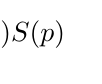
\begin{tikzpicture}
\sbEntree{E}
\sbBloc{sys}{$H_1(p) $}{E}
\sbRelier[$E(p)\quad $]{E}{sys}
\sbBloc{sys2}{$ H_2(p) $}{sys}
\sbRelier{sys}{sys2}
\sbSortie{S}{sys2} 
\sbRelier[$\quad S(p)$]{sys2}{S}

\begin{scope}[xshift=6.25cm]
\draw (0,0) node {$\Leftrightarrow$};
\end{scope}

\begin{scope}[xshift=7cm]
\sbEntree{E}
\sbBloc{sys}{$H_1(p) H_2(p) $}{E}
\sbRelier[$E(p)\quad $]{E}{sys}
\sbSortie{S}{sys} 
\sbRelier[$\quad S(p)$]{sys}{S}
\end{scope}
\end{tikzpicture} 
\end{center}
\end{resultat}


\begin{resultat}[Blocs en parallèle]
\begin{center}
\begin{tikzpicture}
\sbEntree{E}
\sbBloc{sys}{$H_1(p) $}{E}
\sbRelier[$E(p)\quad $]{E}{sys}
\sbSumb{cp}{sys}
\sbRelier{sys}{cp}

\sbDecaleNoeudy[4]{E}{n}
\sbBloc{sys2}{$H_2(p) $}{n}
\sbRelieryx{E-sys}{sys2}
\sbRelierxy{sys2}{cp}

\sbSortie{S}{cp} 
\sbRelier[$\quad S(p)$]{cp}{S}


\begin{scope}[xshift=4cm]
\draw (0,0) node {$\Leftrightarrow$};
\end{scope}

\begin{scope}[xshift=5cm]
\sbEntree{E}
\sbBloc{sys}{$H_1(p) +H_2(p) $}{E}
\sbRelier[$E(p)\quad $]{E}{sys}
\sbSortie{S}{sys} 
\sbRelier[$\quad S(p)$]{sys}{S}
\end{scope}
\end{tikzpicture} 
\end{center}

\end{resultat}


\begin{resultat}[Réduction de boucle -- À MAITRISER PARFAITEMENT]
\begin{center}
\begin{tikzpicture}
\sbEntree{E}
\sbComp{cp}{E}
\sbRelier[$E(p)\quad $]{E}{cp}
\sbBloc{sys}{$H_1(p) $}{cp}
\sbRelier{cp}{sys}
\sbSortie{S}{sys} 
\sbRelier[$\quad S(p)$]{sys}{S}

\sbDecaleNoeudy[4]{cp}{n}
\sbBloc{sys2}{$H_2(p) $}{n}
\sbRelierxy{sys2}{cp}
\sbRelieryx{sys-S}{sys2}
%
%\sbBloc{sys}{$H_1(p) $}{E}
%\sbRelier{E}{sys}
%
%\sbDecaleNoeudy[4]{E}{n}
%\sbBloc{sys2}{$H_2(p) $}{n}
%\sbRelieryx{E-sys}{sys2}
%\sbRelierxy{sys2}{cp}
%
%\sbSortie{S}{cp} 
%\sbRelier[$\quad S(p)$]{cp}{S}


\begin{scope}[xshift=5cm]
\draw (0,0) node {$\Leftrightarrow$};
\end{scope}

\begin{scope}[xshift=6cm]
\sbEntree{E}
\sbBloc{sys}{$\dfrac{H_1(p)}{1+H_1(p)H_2(p)} $}{E}
\sbRelier[$E(p)\quad $]{E}{sys}
\sbSortie{S}{sys} 
\sbRelier[$\quad S(p)$]{sys}{S}
\end{scope}
\end{tikzpicture} 
\end{center}

\end{resultat}


\begin{resultat}[Comparateurs en série]

\begin{center}
\begin{tikzpicture}
\sbEntree{E}
\sbComp{cp1}{E}
\sbComph{cp2}{cp1}
\sbSortie{S}{cp2} 

\sbRelier[$E(p)\quad $]{E}{cp1}
\sbRelier{cp1}{cp2}
\sbRelier[$\quad S(p)$]{cp2}{S}

\sbDecaleNoeudy[4]{E}{n1}
\sbDecaleNoeudy[-4]{E}{n2}
\sbRelierxy[$E_1(p)$]{n1}{cp1}
\sbRelierxy[$E_2(p)$]{n2}{cp2}


\begin{scope}[xshift=5cm]
\draw (0,0) node {$\Leftrightarrow$};
\end{scope}

\begin{scope}[xshift=6cm]
\sbEntree{E}
\sbComph{cp1}{E}
\sbComp{cp2}{cp1}
\sbSortie{S}{cp2} 

\sbRelier[$E(p)\quad $]{E}{cp1}
\sbRelier{cp1}{cp2}
\sbRelier[$\quad S(p)$]{cp2}{S}

\sbDecaleNoeudy[4]{E}{n1}
\sbDecaleNoeudy[-4]{E}{n2}
\sbRelierxy[$E_1(p)$]{n1}{cp2}
\sbRelierxy[$E_2(p)$]{n2}{cp1}
\end{scope}

\end{tikzpicture}
\end{center}
\end{resultat}


\begin{resultat}[Point de prélèvement]
\begin{center}
\begin{tikzpicture}
\sbEntree{E}
\sbBloc{b1}{$H_1(p) $}{E}
\sbSortie{S}{b1} 

\sbRelier[$E(p)\quad $]{E}{b1}
\sbRelier[$\quad S(p)$]{b1}{S}

\sbDecaleNoeudy[4]{S}{n1}
\sbBlocr{b2}{$H_2(p)$}{n1}
\sbRelieryx{b1-S}{b2}
\sbDecaleNoeudx[-4]{b2}{n2}
\sbRelier[$\quad R(p)\quad \quad $]{b2}{n2}

\begin{scope}[xshift=4cm]
\draw (0,0) node {$\Leftrightarrow$};
\end{scope}

\begin{scope}[xshift=8cm]
\sbEntree{E}
\sbBloc{b1}{$H_1(p)$}{E}
\sbSortie{S}{b1} 

\sbRelier[$E(p)\quad $]{E}{b1}
\sbRelier[$\quad S(p)$]{b1}{S}

\sbDecaleNoeudy[4]{E}{n1}
\sbDecaleNoeudx[2]{n1}{n2}
\sbBlocr{b2}{$H_2(p) H_1(p)$}{n2}
\sbRelieryx{E-b1}{b2}
\sbDecaleNoeudx[-6]{b2}{n3}
\sbRelier[$\quad R(p)\quad \quad $]{b2}{n3}
\end{scope}

\end{tikzpicture}
\end{center}

\end{resultat}



\subsection{Fonctions usuelles}

\begin{defi}[Fonction de transfert en boucle fermée -- FTBF]
\textit{Formule de Black}

$$H(p)=\dfrac{S(p)}{E(p)}=\dfrac{H_1(p)}{1+H_1(p)H_2(p)}$$
\end{defi}


\marginnote[-3cm]{\xpComp{SLCI}{08}}

\begin{marginfigure}[-2cm]
\resizebox{\columnwidth}{!}{
\begin{tikzpicture}
\sbEntree{E}
\sbComp{cp}{E}
\sbRelier[$E(p)\quad $]{E}{cp}
\sbBloc[4]{sys}{$H_1(p) $}{cp}
\sbRelier[$\varepsilon(p)$]{cp}{sys}
\sbSortie[4]{S}{sys} 
\sbRelier[$\quad S(p)$]{sys}{S}

\sbDecaleNoeudy[4]{cp}{n}
\sbDecaleNoeudx[2]{n}{n2}
\sbBloc{sys2}{$H_2(p) $}{n2}
\sbRelierxy[$R(p)$]{sys2}{cp}
\sbRelieryx{sys-S}{sys2}
\end{tikzpicture}}
\end{marginfigure}


%\begin{marginfigure}
%\begin{tikzpicture}
%\sbEntree{E}
%\sbComp{cp}{E}
%\sbRelier[$E(p)\quad $]{E}{cp}
%\sbBloc[4]{sys}{$H_1(p) $}{cp}
%\sbRelier[$\varepsilon(p)$]{cp}{sys}
%\sbSortie[4]{S}{sys} 
%\sbRelier[$\quad S(p)$]{sys}{S}
%
%\sbDecaleNoeudy[4]{cp}{n}
%\sbDecaleNoeudx[2]{n}{n2}
%\sbBloc{sys2}{$H_2(p) $}{n2}
%\sbRelierxy[$R(p)$]{sys2}{cp}
%\sbRelieryx{sys-S}{sys2}
%\end{tikzpicture}
%\end{marginfigure}

\begin{defi}[Fonction de transfert en boucle ouverte -- FTBO]

$$\text{FTBO}(p)=\dfrac{R(p)}{\varepsilon(p)}=H_1(p) H_2(p)$$

\end{defi}

%
%\begin{defi}[Chaîne directe] ~\\
%
%\end{defi}
%
%
%
%\begin{defi}[L'écart] ~\\
%
%\end{defi}
%

\begin{defi}[Théorème de superposition]
Soit un système d'entrées $E_1$ et $E_2$ et de sortie $S$. On note $H_1=\dfrac{S}{E_1}$ lorsque $E_2$ est nulle et $H_2=\dfrac{S}{E_2}$ lorsque $E_1$ est nulle. En superposant, on a alors : $S=H_1 E_1 + H_2 E_2$.
\end{defi}



